\documentclass[answers]{exam}
\usepackage{../../mypackages}
\usepackage{../../macros}

%\usepackage{blindtext}

\SolutionEmphasis{\color{blue}}
\renewcommand{\solutiontitle}{\noindent}

\renewcommand{\arraystretch}{1.5} % Augmente l'espacement vertical entre les lignes du tableau
\newcolumntype{C}{>{\centering\arraybackslash}m{2cm}}

\SetLabelAlign{myright}{\hss\llap{$#1$}}
\newlist{where}{description}{1}
\setlist[where]{labelwidth=2cm,labelsep=1em,
                        leftmargin=!,align=myright,font=\normalfont}

\setlength{\parindent}{0pt}

\title{Fiche d'exercices}
\author{N. Bancel}
\date{23 Janvier 2025}

\begin{document}


\textbf{Collège Lycée Suger}
\hfill
\textbf{Physique-Chimie} \\

\textbf{Année 2024-2025}
\hfill
\textbf{3ème Cambridge International} \par

{\let\newpage\relax\maketitle}
%\maketitle


\section*{Lien entre focale et niveau de zoom}

\subsection*{1. Définition de la focale}

La \textbf{focale}, exprimée en millimètres (mm), est la distance entre le centre optique de l'objectif et le capteur lorsque l'image est nette à l'infini. Elle détermine :
\begin{itemize}[noitemsep]
    \item L'\textbf{angle de champ}, c'est-à-dire la portion de la scène visible dans l'image.
    \item L'\textbf{agrandissement}, ou niveau de zoom des objets.
\end{itemize}

\subsection*{2. Relation entre focale et zoom}

\begin{itemize}[noitemsep]
    \item \textbf{Courte focale} (ex. : 18 mm) :
    \begin{itemize}[noitemsep]
        \item Large angle de champ : on capture une grande portion de la scène.
        \item Faible zoom : les objets apparaissent plus petits et plus éloignés.
        \item Usage : paysages, scènes larges.
    \end{itemize}
    \item \textbf{Longue focale} (ex. : 200 mm) :
    \begin{itemize}[noitemsep]
        \item Angle de champ réduit : on capture une petite portion de la scène.
        \item Fort zoom : les objets apparaissent agrandis et rapprochés.
        \item Usage : photographie animalière, sport, portraits isolés.
    \end{itemize}
\end{itemize}

\subsection*{3. Pourquoi une longue focale augmente-t-elle le zoom ?}

Une longue focale concentre les rayons lumineux sur une petite portion du capteur, ce qui agrandit les objets. À l'inverse, une courte focale répartit les rayons lumineux sur une grande surface, ce qui donne une vue plus large et réduit la taille apparente des objets.

\subsection*{4. Récapitulatif}

\begin{itemize}[noitemsep]
    \item \textbf{Courte focale (grand angle)} : Large champ, faible zoom.
    \item \textbf{Longue focale (téléobjectif)} : Champ étroit, fort zoom.
\end{itemize}


\section*{Pour mieux comprendre la notion d'ouverture de diaphragme}


\subsection*{1. Que signifient f/2.8 ou f/8 ?}

Les nombres tels que f/2.8 ou f/8 sont appelés \textbf{valeurs d'ouverture} ou \textbf{nombres f}. Ils indiquent la taille relative de l'ouverture du diaphragme dans l'objectif de l'appareil photo.

\begin{itemize}[noitemsep]
    \item La valeur \( f \) est une fraction : \( f/\text{N} \), où \( f \) est la longueur focale de l'objectif (en mm) et \( \text{N} \) est le diamètre relatif de l'ouverture.
    \item Par exemple :
    \begin{itemize}[noitemsep]
        \item Avec un objectif de 50 mm, une ouverture f/2.8 signifie que le diamètre de l'ouverture est \( 50 \, \text{mm} / 2.8 \approx 17.9 \, \text{mm} \).
        \item Une ouverture f/8 signifie que le diamètre de l'ouverture est \( 50 \, \text{mm} / 8 = 6.25 \, \text{mm} \).
    \end{itemize}
    \item Plus le nombre f est \textbf{petit} (par ex., f/2.8), plus l'ouverture est \textbf{grande} et laisse entrer beaucoup de lumière.
    \item Plus le nombre f est \textbf{grand} (par ex., f/8), plus l'ouverture est \textbf{petite} et laisse entrer moins de lumière.
\end{itemize}

\subsection*{2. Pourquoi ces nombres influencent-ils la profondeur de champ ?}

La \textbf{profondeur de champ} est la zone de netteté de l'image. La taille de l'ouverture du diaphragme influence cette zone :
\begin{itemize}[noitemsep]
    \item Avec une \textbf{grande ouverture} (petit nombre f, comme f/2.8) :
    \begin{itemize}[noitemsep]
        \item La profondeur de champ est \textbf{réduite} : seul le sujet principal est net, tandis que l'arrière-plan (et parfois l'avant-plan) est flou.
        \item Cela est idéal pour isoler le sujet, comme en photographie de portrait.
    \end{itemize}
    \item Avec une \textbf{petite ouverture} (grand nombre f, comme f/8 ou f/16) :
    \begin{itemize}[noitemsep]
        \item La profondeur de champ est \textbf{augmentée} : davantage d'éléments de la scène sont nets, à la fois à l'avant et à l'arrière du sujet.
        \item Cela est utile pour des paysages ou des photos où toute la scène doit être nette.
    \end{itemize}
\end{itemize}

\subsection*{3. Pourquoi cela se produit-il ?}

Cette influence est due à la \textbf{physique optique} :
\begin{itemize}[noitemsep]
    \item Une grande ouverture (f/2.8) fait converger les rayons lumineux sur le capteur avec une plus grande divergence angulaire. Cela rend difficile la mise au point simultanée sur plusieurs plans (avant et arrière du sujet), réduisant la profondeur de champ.
    \item Une petite ouverture (f/8) limite cette divergence angulaire, permettant une meilleure mise au point sur plusieurs plans, ce qui augmente la profondeur de champ.
\end{itemize}

\subsection*{4. Illustration simplifiée : profondeur de champ et ouverture}

Imaginons une scène avec un sujet et un arrière-plan :

\begin{itemize}[noitemsep]
    \item Avec \textbf{f/2.8 (grande ouverture)} : le sujet est net, mais l'arrière-plan est flou. Idéal pour les portraits.
    \item Avec \textbf{f/8 (petite ouverture)} : le sujet et l'arrière-plan sont nets. Idéal pour les paysages.
\end{itemize}

\subsection*{5. Récapitulatif des effets de l'ouverture}

\begin{itemize}[noitemsep]
    \item \textbf{Petit nombre f (ex. : f/2.8)} : Plus de lumière, faible profondeur de champ (arrière-plan flou).
    \item \textbf{Grand nombre f (ex. : f/8)} : Moins de lumière, grande profondeur de champ (plus de netteté globale).
\end{itemize}


\section*{Exercice 5}

\begin{figure}[H]
  \centering
  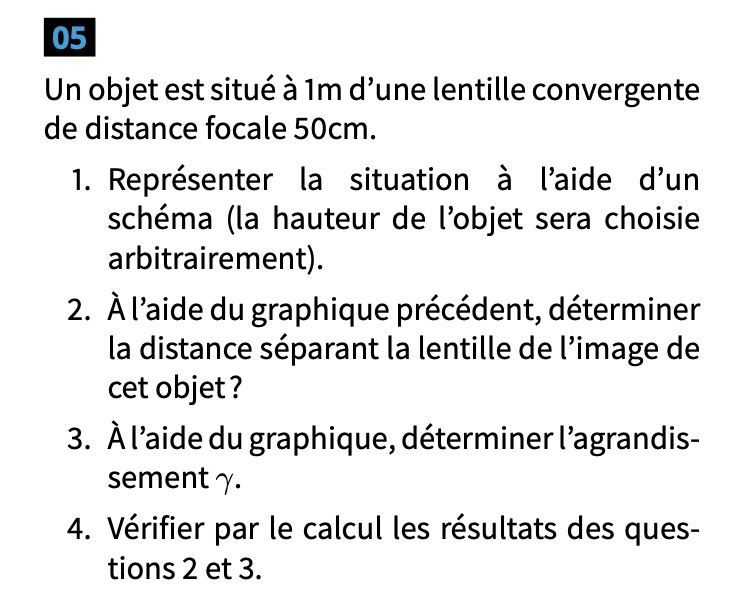
\includegraphics[width=0.7\linewidth]{img/exercice_5.jpg}
\end{figure}



\subsection*{1. Représentation graphique}

Pour représenter la situation, nous traçons un schéma dans un repère orthonormé défini comme suit :
\[
\left(O\mathpunct{} ; \ \overrightarrow{OA}\mathpunct{}, \ \overrightarrow{OB}\mathpunct{}, \ \overrightarrow{OE}\right)
\]
\begin{compactenum}
\item On place la lentille convergente en $O$, son axe optique est $\overrightarrow{OA}$.
\item L'objet est situé à 1m ($d_o = 1~\text{m} = 100~\text{cm}$) à gauche de la lentille.
\item La distance focale $f$ de la lentille est $50~\text{cm}$.
\end{compactenum}

Un schéma doit montrer les rayons caractéristiques :
\begin{compactenum}
    \item Un rayon passant par le centre optique (invariant).
    \item Un rayon parallèle à l'axe optique qui passe par le foyer image.
\end{compactenum}

\subsection*{2. Calcul de la distance lentille-image}

La relation de conjugaison est donnée par :
\[
\frac{1}{f} = \frac{1}{d_o} + \frac{1}{d_i}
\]
où :
\begin{compactenum}
    \item $f = 50~\text{cm}$,
    \item $d_o = 100~\text{cm}$,
    \item $d_i$ est la distance lentille-image que nous cherchons.
\end{compactenum}

Substituons les valeurs dans la formule :
\[
\frac{1}{50} = \frac{1}{100} + \frac{1}{d_i}
\]
\[
\frac{1}{d_i} = \frac{1}{50} - \frac{1}{100}
\]
\[
\frac{1}{d_i} = \frac{2}{100} - \frac{1}{100} = \frac{1}{100}
\]
Ainsi, $d_i = 100~\text{cm} = 1~\text{m}$.

\subsection*{3. Calcul de l’agrandissement $\gamma$}

L'agrandissement $\gamma$ est défini par :
\[
\gamma = \frac{d_i}{d_o}
\]
Substituons les valeurs :
\[
\gamma = \frac{100}{100} = 1
\]
Cela signifie que l'image est renversée et de même taille que l'objet.

\subsection*{4. Vérification des résultats}

\begin{compactenum}
    \item La distance lentille-image calculée est $d_i = 100~\text{cm}$, ce qui est cohérent avec le schéma graphique.
    \item L'agrandissement $\gamma = 1$ confirme que l'image est renversée et de même taille que l'objet, ce qui correspond au schéma.
\end{compactenum}

\noindent Ainsi, les calculs et le graphique sont cohérents.

\section*{Exercice 8}

\begin{figure}[H]
  \centering
  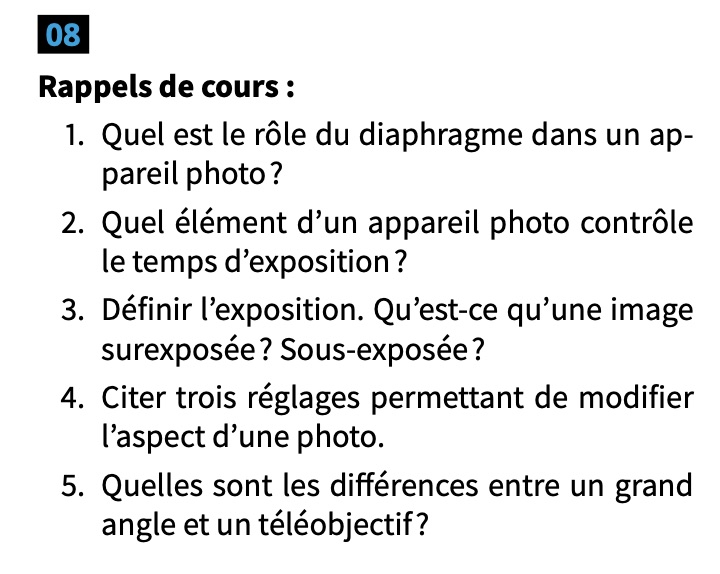
\includegraphics[width=0.7\linewidth]{img/exercice_8.jpg}
\end{figure}

\subsection*{1. Quel est le rôle du diaphragme dans un appareil photo ?}

Le diaphragme contrôle la quantité de lumière qui entre dans l’appareil photo. En ajustant l'ouverture, il permet de :
\begin{compactenum}
    \item Régler la luminosité de l’image.
    \item Modifier la profondeur de champ, c'est-à-dire la zone de netteté dans une photo.
\end{compactenum}

\subsection*{2. Quel élément d’un appareil photo contrôle le temps d’exposition ?}

C’est l’obturateur qui contrôle le temps d’exposition. Il détermine la durée pendant laquelle le capteur (ou la pellicule) est exposé à la lumière. Un temps d’exposition plus long permet de capter plus de lumière, mais augmente le risque de flou si l’appareil ou le sujet bouge.

\subsection*{3. Définir l’exposition. Qu’est-ce qu’une image surexposée ? Sous-exposée ?}

L’exposition correspond à la quantité totale de lumière atteignant le capteur ou la pellicule. Elle est déterminée par trois paramètres : l’ouverture du diaphragme, le temps d’exposition et la sensibilité ISO.

\begin{compactenum}
    \item Une image surexposée est trop lumineuse, avec des zones claires où les détails sont perdus.
    \item Une image sous-exposée est trop sombre, avec des zones obscures où les détails sont invisibles.
\end{compactenum}

\subsection*{4. Citer trois réglages permettant de modifier l’aspect d’une photo.}

Trois réglages principaux influencent l’aspect d’une photo :
\begin{compactenum}
    \item L’ouverture du diaphragme, qui affecte la luminosité et la profondeur de champ.
    \item La vitesse d’obturation, qui contrôle le flou de mouvement et la luminosité.
    \item La sensibilité ISO, qui modifie la luminosité et le grain de l’image.
\end{compactenum}

\subsection*{5. Quelles sont les différences entre un grand angle et un téléobjectif ?}

\begin{compactenum}
    \item Un grand angle a une courte focale et offre un large champ de vision. Il est utilisé pour des paysages ou des scènes où l’on veut capturer beaucoup d’éléments.
    \item Un téléobjectif a une longue focale et un champ de vision réduit. Il est idéal pour capturer des sujets éloignés, comme en photographie animalière ou sportive.
\end{compactenum}


\section*{Exercice 13}

\begin{figure}[H]
  \centering
  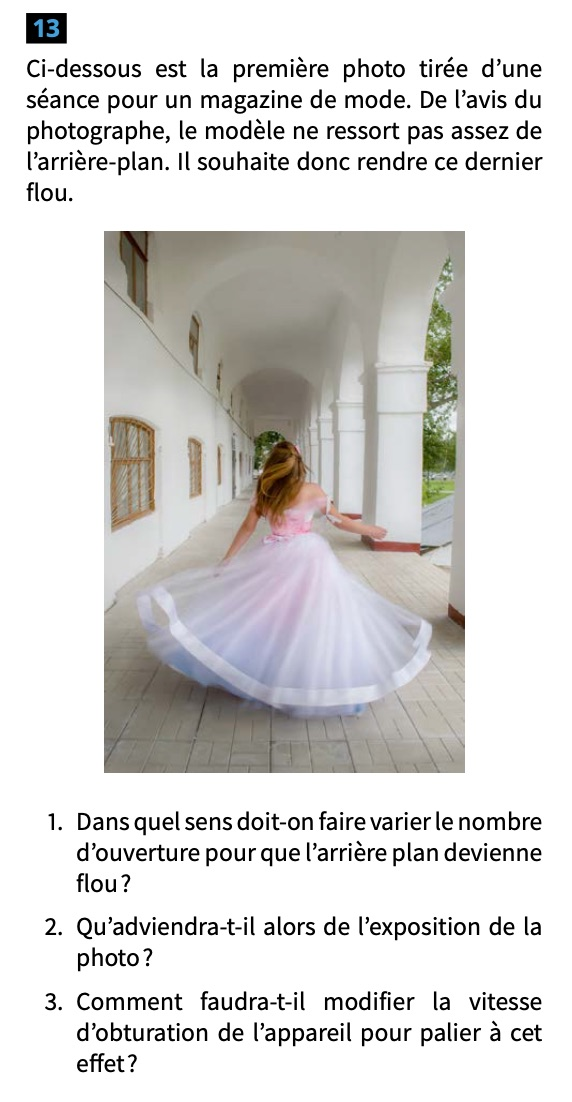
\includegraphics[width=0.7\linewidth]{img/exercice_13.jpg}
\end{figure}

\subsection*{1. Dans quel sens doit-on faire varier le nombre d'ouverture pour que l'arrière-plan devienne flou ?}

Pour rendre l'arrière-plan flou, il faut diminuer le nombre d'ouverture (augmenter l'ouverture du diaphragme). Une ouverture plus grande (par exemple, f/2.8 au lieu de f/8) réduit la profondeur de champ, ce qui permet de flouter l'arrière-plan et de mieux isoler le sujet.

\subsection*{2. Qu'adviendra-t-il alors de l'exposition de la photo ?}

En augmentant l'ouverture du diaphragme, davantage de lumière entre dans l'appareil photo. Cela rend la photo plus lumineuse, ce qui peut entraîner une surexposition si aucun autre paramètre n'est ajusté.

\subsection*{3. Comment faudra-t-il modifier la vitesse d'obturation de l'appareil pour pallier à cet effet ?}

Pour compenser l'augmentation de lumière due à une ouverture plus grande, il faut réduire le temps d'exposition en augmentant la vitesse d'obturation. Cela signifie utiliser une vitesse plus rapide (par exemple, passer de 1/100 s à 1/500 s) pour éviter une surexposition tout en conservant une bonne luminosité dans l'image.


\section*{Correction de l'exercice 14}


\begin{figure}[H]
  \centering
  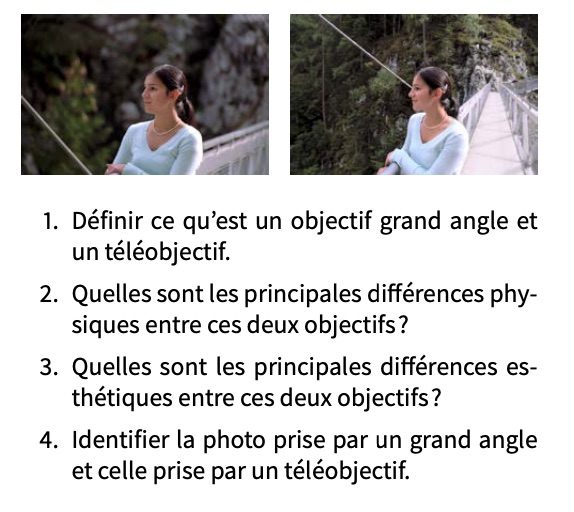
\includegraphics[width=0.7\linewidth]{img/exercice_14.jpg}
\end{figure}

\subsection*{1. Définir ce qu'est un objectif grand angle et un téléobjectif}

\begin{itemize}
    \item Un \textbf{objectif grand angle} a une courte focale (par exemple, 18 mm). Il offre un large champ de vision, idéal pour capturer des paysages ou des scènes où de nombreux éléments doivent apparaître dans le cadre.
    \item Un \textbf{téléobjectif} a une longue focale (par exemple, 200 mm). Il permet de zoomer sur des sujets éloignés en réduisant le champ de vision. Il est souvent utilisé en photographie animalière ou sportive.
\end{itemize}

\subsection*{2. Quelles sont les principales différences physiques entre ces deux objectifs ?}

\begin{compactenum}
    \item Un objectif grand angle est généralement plus court et compact.
    \item Un téléobjectif est souvent plus long, plus lourd, et son diamètre d'ouverture peut être plus large pour compenser la perte de lumière.
    \item Les lentilles internes des téléobjectifs sont conçues pour capturer et rapprocher des sujets distants, tandis que les objectifs grand angle optimisent la captation d'un champ de vision étendu.
\end{compactenum}

\subsection*{3. Quelles sont les principales différences esthétiques entre ces deux objectifs ?}

\begin{compactenum}
    \item Le \textbf{grand angle} déforme légèrement les perspectives, ce qui donne une impression de profondeur accrue. Par exemple, les objets proches paraissent plus grands, tandis que les objets éloignés paraissent très petits.
    \item Le \textbf{téléobjectif} compresse les perspectives, ce qui rapproche visuellement les différents plans d'une scène. Cela crée une image plus plate, mais met mieux en valeur les sujets isolés.
    \item Le grand angle capte un arrière-plan large et détaillé, tandis que le téléobjectif tend à flouter davantage l'arrière-plan, ce qui met en valeur le sujet principal.
\end{compactenum}

\subsection*{4. Identifier la photo prise par un grand angle et celle prise par un téléobjectif}

\begin{itemize}
    \item La première photo (à gauche) est prise avec un \textbf{téléobjectif}, car elle montre une compression des plans et un flou d'arrière-plan, isolant bien le sujet.
    \item La seconde photo (à droite) est prise avec un \textbf{grand angle}, car elle montre un champ de vision large et une plus grande profondeur de champ, incluant de nombreux détails de l'arrière-plan.
\end{itemize}


\section*{Correction de l'exercice 15}


\begin{figure}[H]
  \centering
  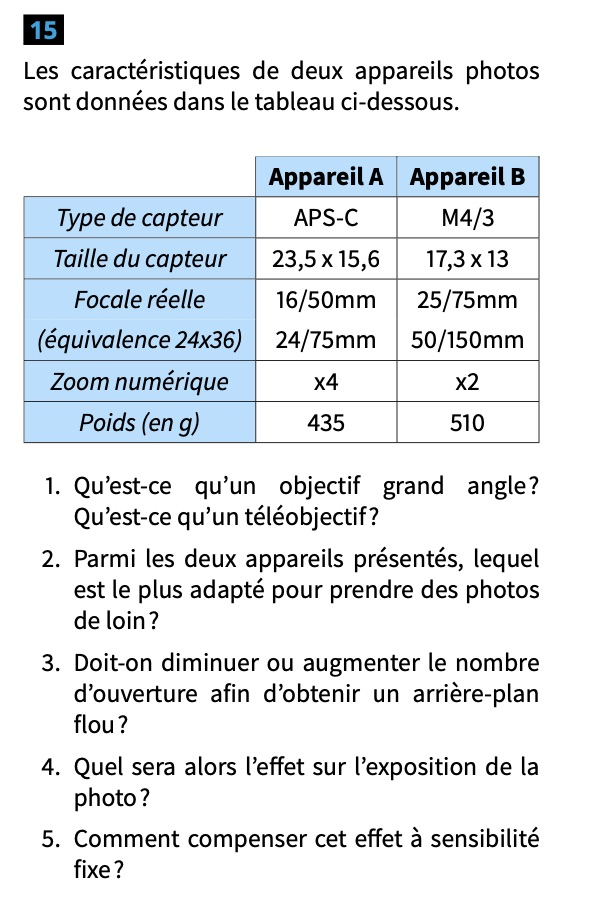
\includegraphics[width=0.7\linewidth]{img/exercice_15.jpg}
\end{figure}

\subsection*{1. Qu'est-ce qu'un objectif grand angle ? Qu'est-ce qu'un téléobjectif ?}

\begin{itemize}
    \item Un \textbf{objectif grand angle} possède une courte focale, typiquement inférieure à 35 mm (équivalence 24x36). Il offre un large champ de vision, idéal pour des paysages ou des scènes où plusieurs éléments doivent être capturés.
    \item Un \textbf{téléobjectif} possède une longue focale, généralement supérieure à 70 mm (équivalence 24x36). Il est conçu pour photographier des sujets éloignés, en isolant efficacement le sujet principal.
\end{itemize}

\subsection*{2. Parmi les deux appareils présentés, lequel est le plus adapté pour prendre des photos de loin ?}

L'\textbf{Appareil B} est plus adapté pour les photos de loin car :
\begin{itemize}
    \item Il offre une focale réelle allant jusqu'à 75 mm (équivalent 150 mm en 24x36), ce qui est idéal pour les prises de vue à distance.
    \item Bien que l'Appareil A possède un zoom numérique x4, cela peut entraîner une perte de qualité, alors que l'Appareil B privilégie une focale plus longue sans dépendre d'un fort agrandissement numérique.
\end{itemize}

\subsection*{3. Doit-on diminuer ou augmenter le nombre d'ouverture afin d'obtenir un arrière-plan flou ?}

Pour obtenir un arrière-plan flou, il faut \textbf{diminuer le nombre d'ouverture} (augmenter l'ouverture du diaphragme). Par exemple, passer d'une ouverture f/8 à une ouverture f/2.8 réduit la profondeur de champ et floute l'arrière-plan.

\subsection*{4. Quel sera alors l'effet sur l'exposition de la photo ?}

En augmentant l'ouverture (en diminuant le nombre f), davantage de lumière atteint le capteur, ce qui peut rendre la photo \textbf{suro-exposée} si aucun autre réglage n'est ajusté.

\subsection*{5. Comment compenser cet effet à sensibilité fixe ?}

Pour compenser cet effet sans modifier la sensibilité ISO, il faut :
\begin{itemize}
    \item \textbf{Augmenter la vitesse d'obturation} : réduire le temps d'exposition (par exemple, passer de 1/100 s à 1/500 s).
    \item \textbf{Utiliser un filtre ND (neutral density)} : cela réduit la quantité de lumière entrant dans l'objectif sans affecter les autres réglages.
\end{itemize}

\section*{Exercice165}

\begin{figure}[H]
  \centering
  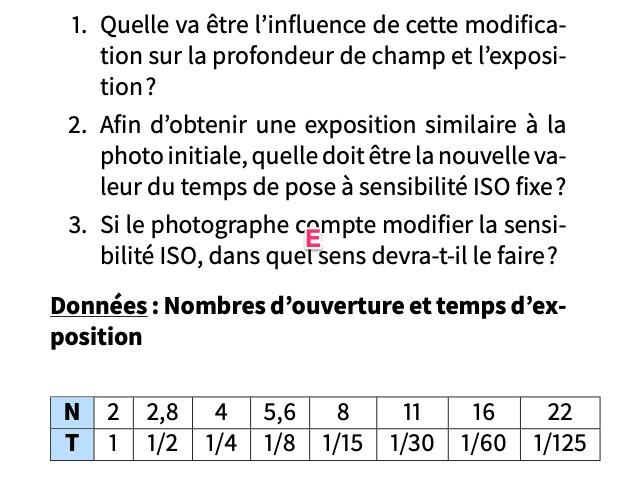
\includegraphics[width=0.7\linewidth]{img/exercice_16.jpg}
\end{figure}


\subsection*{1. Quelle va être l'influence de cette modification sur la profondeur de champ et l'exposition ?}

\begin{itemize}
    \item En passant de \( N = 4 \) à \( N = 8 \) (augmentation du nombre d'ouverture), l'ouverture du diaphragme diminue, ce qui :
    \begin{itemize}
        \item \textbf{Augmente la profondeur de champ} : davantage de plans seront nets dans l'image.
        \item \textbf{Réduit l'exposition} : moins de lumière atteint le capteur, rendant la photo plus sombre si aucun autre paramètre n'est ajusté.
    \end{itemize}
\end{itemize}

\subsection*{2. Afin d'obtenir une exposition similaire à la photo initiale, quelle doit être la nouvelle valeur du temps de pose à sensibilité ISO fixe ?}

La relation entre le nombre d'ouverture (\( N \)) et le temps d'exposition (\( T \)) suit une progression connue. Lorsque le nombre d'ouverture est doublé (par exemple, de \( N = 4 \) à \( N = 8 \)), la quantité de lumière entrant est divisée par 4. Pour compenser, le temps de pose doit être multiplié par 4.

\begin{itemize}
    \item Initialement, \( N = 4 \) et \( T = 1/30 \).
    \item Avec \( N = 8 \), le temps de pose devient :
    \[
    T_{\text{nouveau}} = T_{\text{initial}} \times 4 = \frac{1}{30} \times 4 = \frac{4}{30} = \frac{2}{15} \approx 1/8 \, \text{(s)}.
    \]
\end{itemize}
Ainsi, le nouveau temps de pose doit être \( \mathbf{1/8} \, \text{s} \).

\subsection*{3. Si le photographe compte modifier la sensibilité ISO, dans quel sens devra-t-il le faire ?}

Si le photographe préfère ne pas modifier le temps de pose mais souhaite conserver la même exposition, il peut ajuster la sensibilité ISO.

\begin{itemize}
    \item En augmentant le nombre d'ouverture (\( N = 8 \)), moins de lumière atteint le capteur.
    \item Pour compenser ce déficit, il doit \textbf{augmenter la sensibilité ISO}. Une sensibilité plus élevée rend le capteur plus réactif à la lumière, ce qui rétablit l'exposition initiale.
\end{itemize}

\subsection*{Tableau des données}

Voici les données fournies pour les nombres d'ouverture (\( N \)) et les temps d'exposition (\( T \)) :

\[
\begin{array}{|c|c|c|c|c|c|c|c|c|}
\hline
N & 2 & 2,8 & 4 & 5,6 & 8 & 11 & 16 & 22 \\
\hline
T & 1/2 & 1/4 & 1/8 & 1/15 & 1/30 & 1/60 & 1/125 & 1/250 \\
\hline
\end{array}
\]

\end{document}
